\section{Theoretische Grundlagen}

\subsection{Zerfallsgesetz}

Radioaktive Zerfälle können durch das Zerfallsgesetz beschrieben werden:
\begin{gather}
 \frac{dP}{dt} = \lambda \\
 \frac{dN}{dt} = - \lambda N(t) = - A(t) \label{dNdtlambdaN}\\
 N(t) = N_0 e^{-\lambda t}
\end{gather}

Daraus ergibt sich auch die Halbwertszeit:
\begin{gather}
 N(t_{1/2}) = \frac{1}{2} N_0 = N_0 e^{-\lambda t_{1/2}} \\
 \frac{1}{2} = e^{-\lambda t_{1/2}} \\
 \ln \frac{1}{2} = - \lambda t_{1/2} \\
 t_{1/2} = \frac{\ln 2}{\lambda} \label{t12ln2lambda}\\
\end{gather}


\subsection{$\alpha$-Zerfall}
Als $\alpha$-Zerfall bezeichnet man den Zerfall eines Atoms, bei dem ein \atom{4}{2}{He} Ion den Kern verlässt. Die Reaktionsgleichung lautet also:
$$ \atom{A}{Z}{X} \rightarrow \atom{A-4}{Z-2}{Y}^{-2} + \atom{4}{2}{He}^{+2} $$

\atom{4}{2}{He} besitzt sowohl eine voll besetzte Neutronen- als auch eine voll besetzte Protononenschale, man bezeichnet es auch als "`doppelt magisch"', und hat somit eine sehr hohe Bindungsenergie. Klassisch betrachtet kann ein solches Ion den Atomkern dennoch nicht verlassen, da seine Energie niedriger ist als die des Coulombwalls. Quantenmechanisch ist dies natürlich durch den Tunneleffekt durchaus möglich. Die Wahrscheinlichkeit für einen $\alpha$-Zerfall ergibt sich aus dem Produkt der Einzelwahrscheinlichkeiten für die Bildung eines solchen Ions, seine Rate der "`Wallberührung"' sowie schließlich der Tunnelwahrscheinlichkeit:
$$ W = W_0 \times W_1 \times T $$
Die Tunnelwahrscheinlichkeit $T$ kann mit den Gamow-Faktor $G$ näherungsweise analytisch berechnet werden.

Die Energie des $\alpha$-Teilchens ergibt sich aus der Energiedifferenz zwischen Mutteratom und Tochteratom. Diese unterscheidet sich bei Zerfällen des selben Isotops höchstens durch angeregte Kernzustände. Beim Übergang vom angeregten Mutteratom zum Grundzustand des Tochteratoms erhält das Ion die höchste Energie, beim Übergang von Grundzustand zu Grundzustand ist sie etwas niedriger und für den Übergang von Grundzustand zu angeregtem Tochteratom ist sie am niedrigsten.

Da es also nur endlich viele diskrete Übergangsmöglichkeiten gibt, ist auch das Energiespektrum des $\alpha$-Zerfalls diskret.  

\subsection{$\beta$ - Zerfall}
Als $\beta$-Zerfall bezeichnet man den Übergang eines Protonen zu einem Neutronen oder eines Neutrons zu einem Proton. Der $\beta^-$-Zerfall wird beschrieben durch:
$$ \atom{A}{Z}{X} \rightarrow \atom{A}{Z+1}{Y} + e^- + \overline{\nu} $$
also
$$ n \rightarrow p + e^- + \overline{\nu_e} $$
Der $\beta^+$-Zerfall ist der Zerfall eines Protons in ein Neutron:
$$p \rightarrow n + e^+ + \nu_e$$

\subsection{Elektroneneinfang}

Als weitere Art des $\beta$-Zerfall zählt man noch den Elektroneneinfang (EC, \emph{electron capture)}. Dieser kann stattfinden, wenn ein Elektron der untersten Schale (K-Schale), wegen dessen Aufenthaltswahrscheinlichkeit im Kern, vom Kern eingefangen wird und mit einem Proton zu einem Neutron kombiniert unter Emission eines Elektronenneutrinos:

$$ EC: p^+ + e^- \rightarrow n^0 + \nu_e $$

Der Elektroneneinfang gewinnt mit größeren Kernzahlen an Bedeutung, da dann die Aufenthaltswahrscheinlichkeit im Kern immer größer wird.


\subsection{$\gamma$-Strahlung}

Beim $\alpha$- und $\beta$-Zerfall gehen die Mutterkerne immer mit bestimmten Wahrscheinlichkeiten in verschiedene Energiezustände der Tochterkerne über. Letztere zerfallen innerhalb einer sehr kurzen Zeit ($\sim 10^-9 bis 10^-12 s$) in den Grundzustand. Dabei wird entweder ein Photon emittiert, genannt $\gamma$-Quant, oder es findet \paragraph{Innere Konversion} statt. Die Energie des Kerns geht an ein Hüllenelektron, welches dadurch das Atom mit der verbleibenden Energie als kinetische Energie verlässt. Diese Elektronenlücke wird durch ein Elektron aus einer höheren Schale ersetzt, welches seine überschüssige Energie durch ein Photon (bei schweren Elementen) oder den \paragraph{Auger-Effekt} (bei leichten Elementen) abgiebt.
Dies bedeutet, dass die überschüssige Energie wiederum an ein Elektron abgegeben wird, welches dadurch das Atom verlässt und damit ein zweites Loch im Atom hinterlässt.

\subsection{Wechselwirkung von geladenen Teilen mit Materie}
\subsubsection{Wechselwirkung von Photonen mit Materie}

\subsubsection{Das Absorptionsgesetz}

Ein Photonenstrahl der einfallenden Intensität $I_0$ nimmt exponentiell mit der Dicke x einer durchquerten Materieschicht an Intensität ab. Es gilt also:

$$ I = I_0\cdot e^{-\mu x} $$

wobei $\mu$ der mediumabhängige (und photonenenergieabhängige) Absorptionkoeffizient ist. $\mu$ lässt sich als Summe der Absorptionskoeffizienten aller möglichen Wechselwirkungen von Photonen mit Materie schreiben, nämlich des Photoeffekts, des Compton-Effekts und der Paarbildung.

$$\mu = \mu_{Ph.} + \mu_{C} + \mu_{PB} $$

\subsubsection{Der Photoeffekt}

\begin{figure}[H]
	\begin{minipage}{0.59\textwidth}
	\centering% 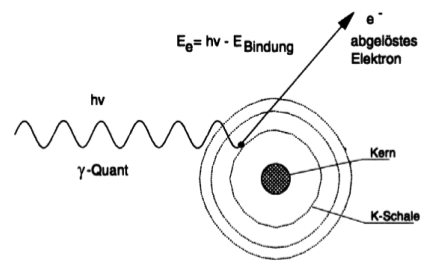
\includegraphics[width=\textwidth]{Bilder/Photoeffekt.png}
	\caption{Photoeffekt}
	\end{minipage}
	\begin{minipage}{0.4\textwidth}
	Wenn ein $\gamma$-Quant ein Elektron aus der Atomhülle herausschlägt, spricht man vom Photoeffekt. Dieser Effekt tritt nur an gebundenen Elek\-tro\-nen auf. Die Energie des Photons geht zum größten Teil auf das Elektron, ein Teil wird jedoch als Rückstoßenergie vom Atom aufgenommen. Die Ab\-sorp\-tions\-wahrscheinlichkeit ist am größten in der K-Schale, also näher beim Kern. Der Photoeffekt dominiert gegenüber den anderen Effekten vor allem bei großen Atomen und Energien unter 100keV des Photons. Die entstandene Lücke wird dann durch ein weniger stark gebundenes oder freies Elektron aufgefüllt, wobei die Differenz der Bindungsenergien als Photon emittiert wird.
	\end{minipage}
\end{figure}

\subsubsection{Der Compton-Effekt}

\begin{figure}[H]
	\begin{minipage}{0.4\textwidth}
	Trifft ein Photon auf ein leicht gebundenes oder freies Elektron, so wird das Photon nicht ganz absorbiert, sondern gibt einen Teil seiner Energie an das Elektron ab und wird selbst gestreut. Durch die Streuung verliert das Photon somit an Energie, d.h. die Frequenz des gestreuten Quants ist kleiner. Der Compton-Effekt dominiert bei Energien zwischen 100 keV und einigen MeV.
	\end{minipage}
	\begin{minipage}{0.59\textwidth}
	\centering %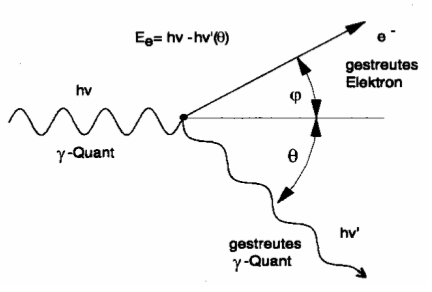
\includegraphics[width=\textwidth]{Bilder/Comptoneffekt.png}
	\caption{Comptoneffekt}
	\end{minipage}

\end{figure}

\subsubsection{Die Paarbildung}

\begin{figure}[H]
	\begin{minipage}{0.49\textwidth}
	\centering %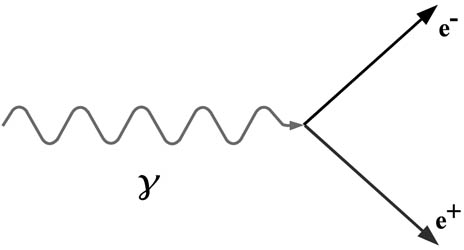
\includegraphics[width=\textwidth]{Bilder/Paarbildung.jpg}
	\caption{Paarbildung}
	\end{minipage}
	\begin{minipage}{0.5\textwidth}
	Hat der $\gamma$-Quant mindestens die doppelte Ruheenergie eines Elektrons, also 1.022 MeV, so kann dieses im Feld eines Atomkerns (Stoßpartner für die Energie-Impuls-Erhaltung) ein Elektron-Positron-Paar erzeugen. Das Positron kann in Anwesenhait von Materie nicht frei existieren und wird abgebremst und annihiliert mit einem Elektron zu 2 bis 3 $\gamma$-Quanten. Im wahrscheinlicheren Fall zweier Quanten, erhalten diese jeweils eine Energie von 511 keV und bewegen sich in einem Winkel von 180$^\circ$ relativ zueinander (wegen Impulserhaltung).
	\end{minipage}
\end{figure}

\subsubsection{Wechselwirkung von Elektronen mit Materie}

\subsection{Absorption und Reichweite radioaktiver Strahlung}
 --> z.T. in Szinti

\subsection{Durchflusszählrohr}
\begin{figure}[H]
 \centering 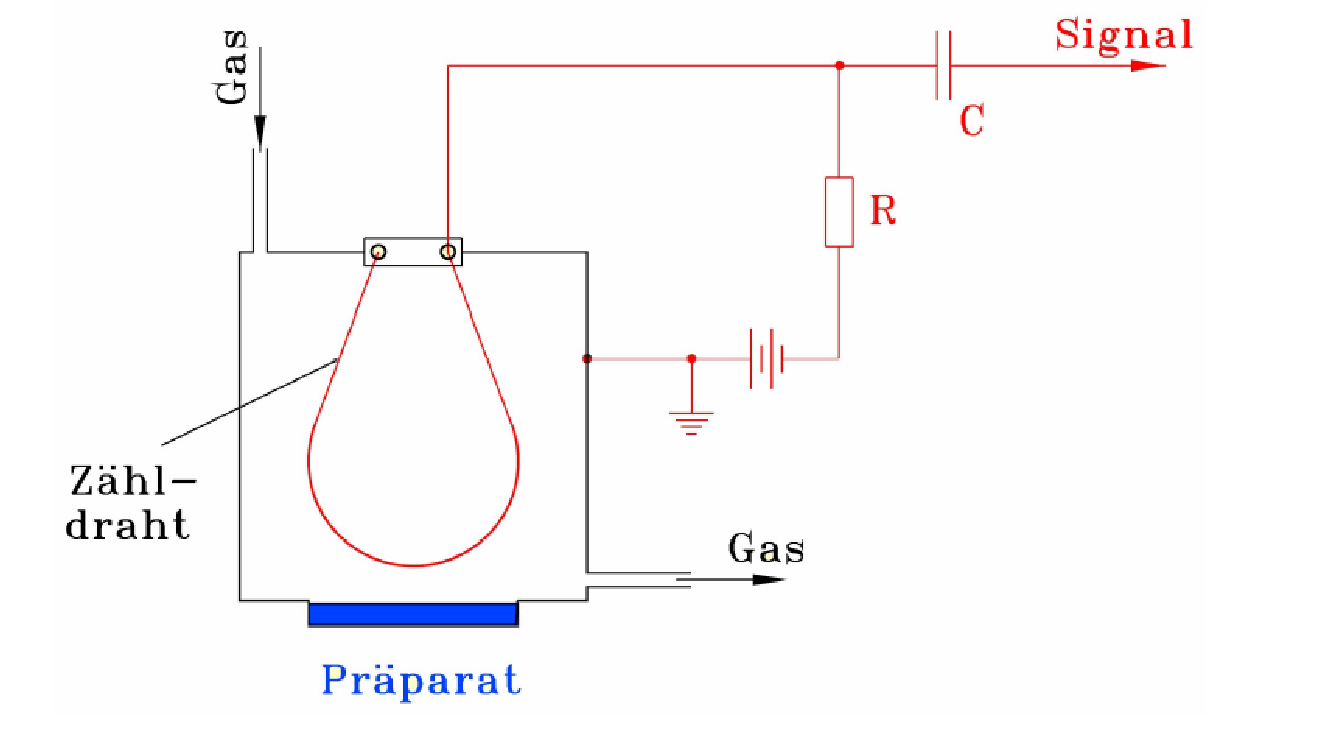
\includegraphics[width=0.9\linewidth]{Bilder/zaehlrohr.png}
 \caption{Aufbau eines Durchflusszählrohrs}
 \label{durchflusszaehlrohr}
\end{figure}
Ein Durchflusszählrohr (siehe Abbildung \ref{durchflusszaehlrohr}) besteht aus einer Zählkammer, die einem normalen Zählrohr ähnelt. Sie besteht also aus einem leitfähigen Kasten und einem Zählring, zwischen denen eine Spannung anliegt. Durch eine Drehvorrichtung kann die Probe direkt in diese Kammer eingebracht werden, wodurch Abschirmungsverluste vermieden werden. Die $alpha$-Teilchen bzw. Elektronen und Positronen des Zerfalls erzeugen nun einen Strompuls am Ring, der detektiert werden kann. In Abhängigkeit von der Spannung gibt es dabei unterschiedliches Verhalten:
\begin{figure}[H]
 \centering 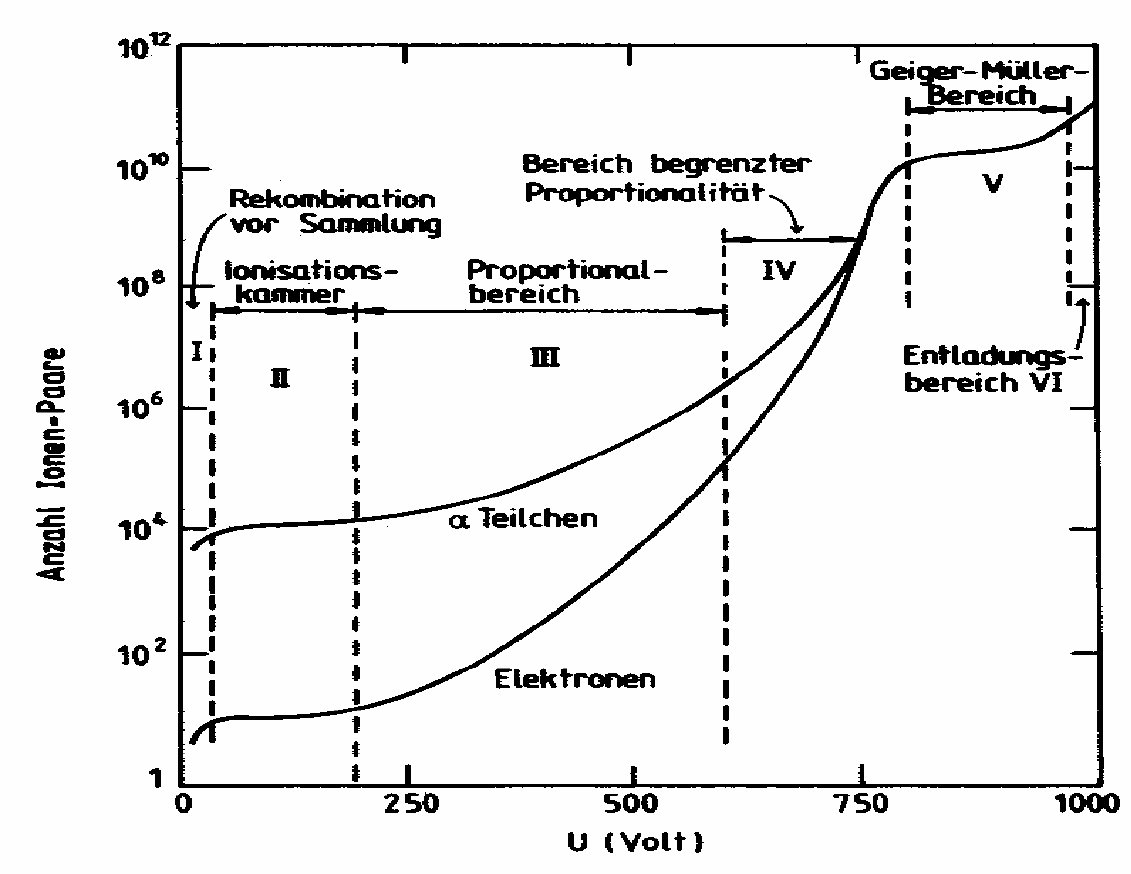
\includegraphics[width=0.9\linewidth]{Bilder/zaehlrohrcharakteristik.png}
 \caption{Typische Zählrohrcharakteristik ( nach ???)}
\end{figure}
\paragraph{Bereich I} Die erzeugten Ionenpaare gelangen nur teilweise bis zum Draht, es kommt meist bereits vorher zur Rekombination. Der gemessene Strom ist hier hauptsächlich von der Spannung abhängig.
\paragraph{Bereich II - Ionisationskammer} Es werden sämtliche Ionenpaare, die durch die Primärionisation entstanden sind, registriert. Man verwendet diesen Spannungsbereich als Ionisationskammer.
\paragraph{Bereich III - Proportionalbereich} Die Ionen aus Primärionisation stoßen mit weiteren Gasmolekülen. Diese werden dadurch ebenfalls ionisiert und es findet eine sogenannte "`Gasverstärkung"' statt. Diese ist proportional zur Energie der Primärteilchen.
\paragraph{Bereich IV} Die Proportionalität zur Primärionisationsenergie wird schwächer.
\paragraph{Bereich V - Geiger-Müller-Bereich} Ein einzelnes Ereigniss löst in diesem Bereich bereits eine Entladungslawine aus und sämtliche Gasatome werden ionisiert. Diese hohe Empfindlichkeit wird im Geiger-Müller-Zählrohr ausgenutzt. 
\paragraph{Bereich VI - Gasentladung} Der Stromfluss bricht in diesem Bereich nicht mehr von selbst ab, ein Zählen der Ereignisse ist somit nichtmehr möglich.

Beim Durchflusszählrohr strömt möglichst konstant ein Gas durch die Kammer, dieses beseitigt verbleibende Ionen vom vorherigen Zählvorgang und verbessert somit die Genauigkeit durch Verringerung der Totzeit und Vermeidung von Fehlzählungen.


























